\chapter{IMU Variances Test} \label{app:IMUVariances}

\textbf{Name: Group 832}\\
\textbf{Date: 06/04/2017}

\subsubsection{Purpose}
Find the variance and bias of the gyroscope present in the IMU, as well as the variance when calculation the attitude using the accelerometer and the magnetometer as described in \autoref{sec:attFusion} in \autoref{eq:roll_acc}, \ref{eq:roll_acc} and \ref{eq:yaw_mag}.

\subsubsection{Procedure}
\subsubsection{Results}

\begin{figure}[H]
    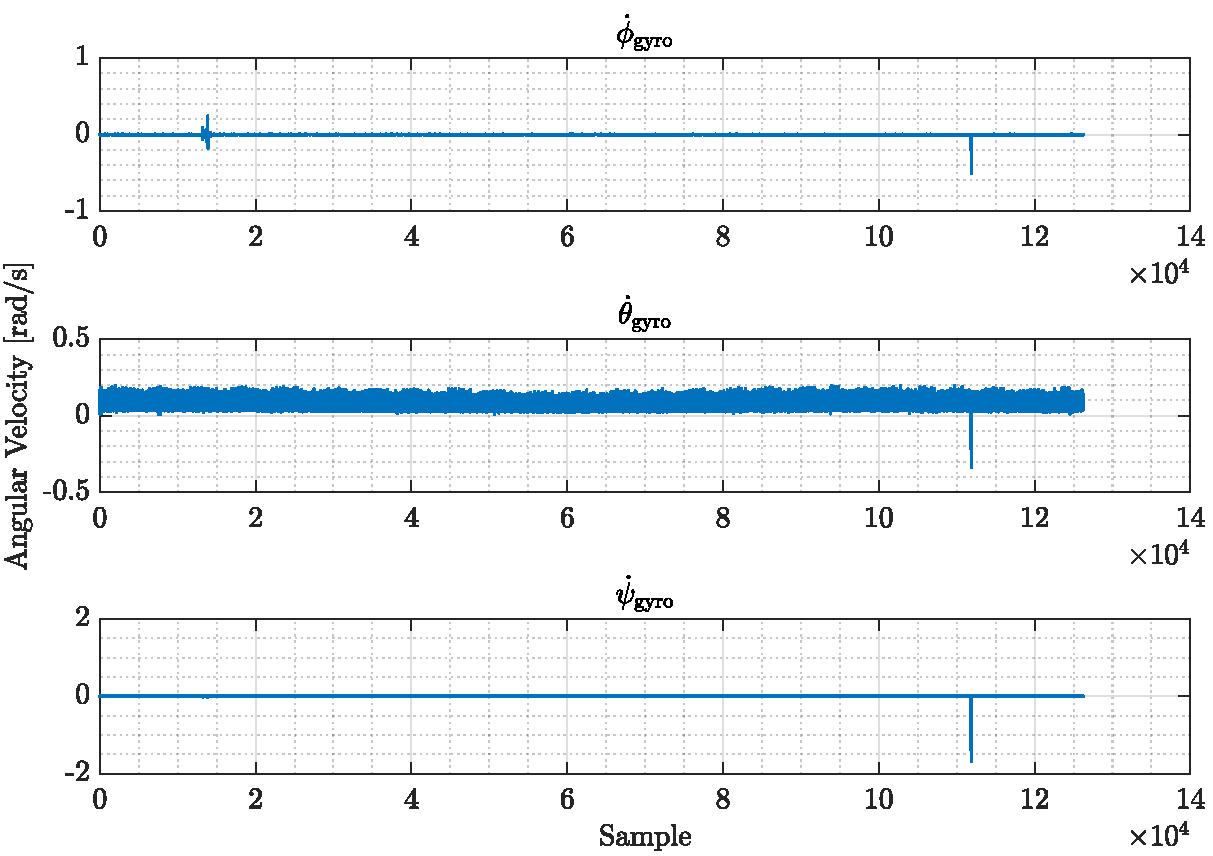
\includegraphics[width=.8\textwidth]{figures/IMUVariancesGyro.pdf}
\end{figure}
\begin{flalign}
     \sigma_{\dot{\phi}\mathrm{,gyro}}^2 & = 0.00001165 \ \mathrm{rad}^2 \mathrm{s}^{-2} \nonumber \\
     \sigma_{\dot{\theta}\mathrm{,gyro}}^2 & = 0.00002264 \ \mathrm{rad}^2 \mathrm{s}^{-2} \nonumber \\
     \sigma_{\dot{\psi}\mathrm{,gyro}}^2 & = 0.00779047  \ \mathrm{rad}^2 \mathrm{s}^{-2} \nonumber
\end{flalign}

\begin{flalign}
    \mathrm{bias}_{\dot{\phi}\mathrm{,gyro}} & = -0.03753197 \ \mathrm{rad s}^{-1} \nonumber \\
    \mathrm{bias}_{\dot{\theta}\mathrm{,gyro}} & = -4.49556388 \ \mathrm{rad s}^{-1} \nonumber \\
    \mathrm{bias}_{\dot{\psi}\mathrm{,gyro}} & = 0.16183876  \ \mathrm{rad s}^{-1} \nonumber
\end{flalign}

\begin{figure}[H] 
    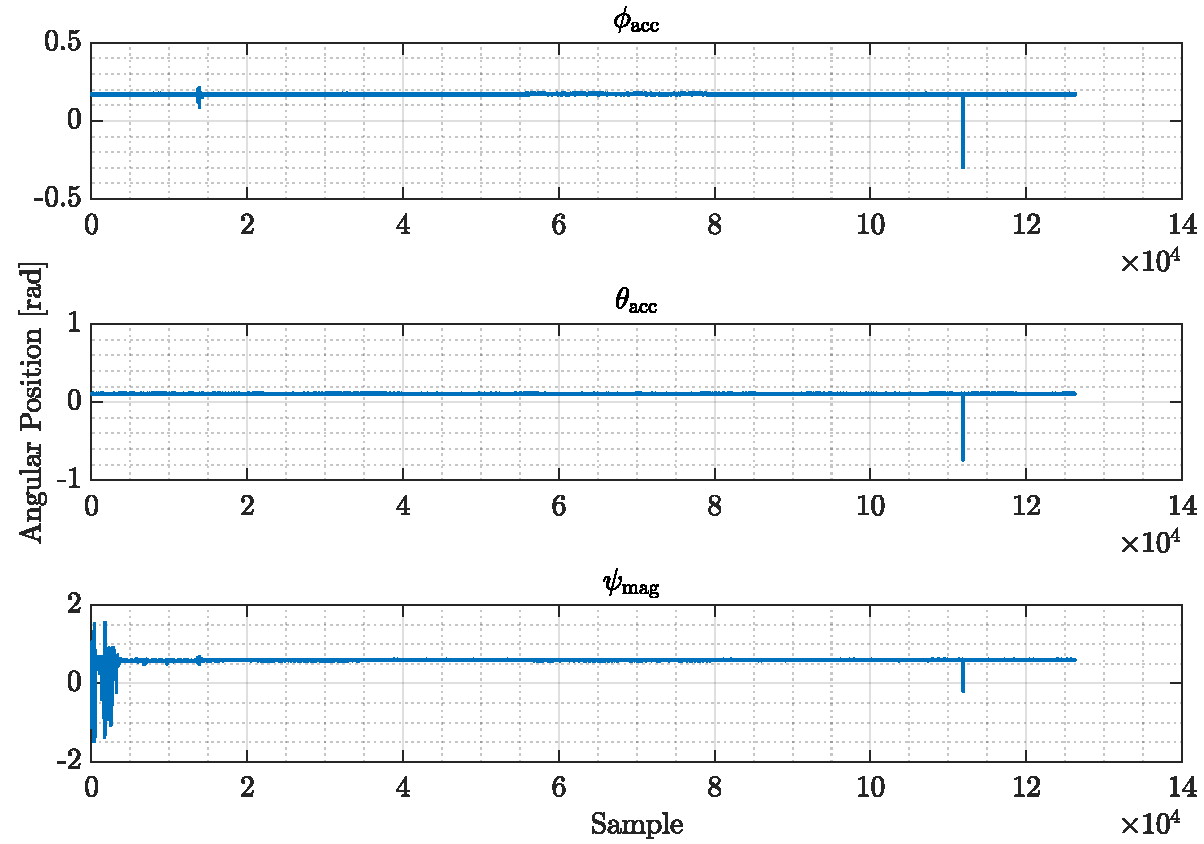
\includegraphics[width=.8\textwidth]{figures/IMUVariancesAtt.pdf}
\end{figure}

\begin{flalign}
    \sigma_{\phi\mathrm{,acc}}^2 & = 0.01033366 \ \mathrm{rad}^2 \nonumber \\
    \sigma_{\theta\mathrm{,acc}}^2 & = 3.98535412 \ \mathrm{rad}^2\nonumber \\
    \sigma_{\psi\mathrm{,mag}}^2 & = 0.03143813 \ \mathrm{rad}^2 \nonumber
\end{flalign}
